\chapter[Studie und Auswertung]{Studie zur Erhebung multimodaler Interaktionszeiten und Auswertung}\label{cha:Studie}
In diesem Kapitel wird das Studiendesign und die Durchführung der Studie beschrieben, sowie auf die anschließende Auswertung eingegangen. 
\section[Studiendesign]{Studiendesign zur Erhebung multimodaler Interaktionszeiten}
Für die Studie verwenden wir ein Within Subject Design, bei dem jeder Proband alle Kombinationen der vier Anwendungsbeispiele im stehenden Auto durchführen soll.
\subsection[Permutation]{Permutation der Anwendungsbeispiele}
Mit einem festgelegten Moduswechsel und drei verschiedenen Modalitäten (Touch, Gestik und Sprache) kommen wir auf neun Kombinationen pro Anwendungsbeispiel. 
Eine Ausnahme ist das Navigationsanwendungsbeispiel, bei dem wir uns entschieden haben die Zieleingabe nicht für die Gestik umzusetzen. 
Somit fallen die Varianten Geste \& Geste, Sprache \& Geste und Touch \& Geste weg. 
Damit kommen wir bei diesem Anwendungsbeispiel lediglich auf sechs multimodale Kombinationen. 
Zu den multimodalen Varianten testen wir auch die drei unimodalen Varianten der vier Anwendungsbeispiele und kommen insgesamt auf 33 Varianten für alle vier Anwendungsbeispiele, die jeder Proband durchzuführen hat. 
\begin{figure}[ht]
  \centering
  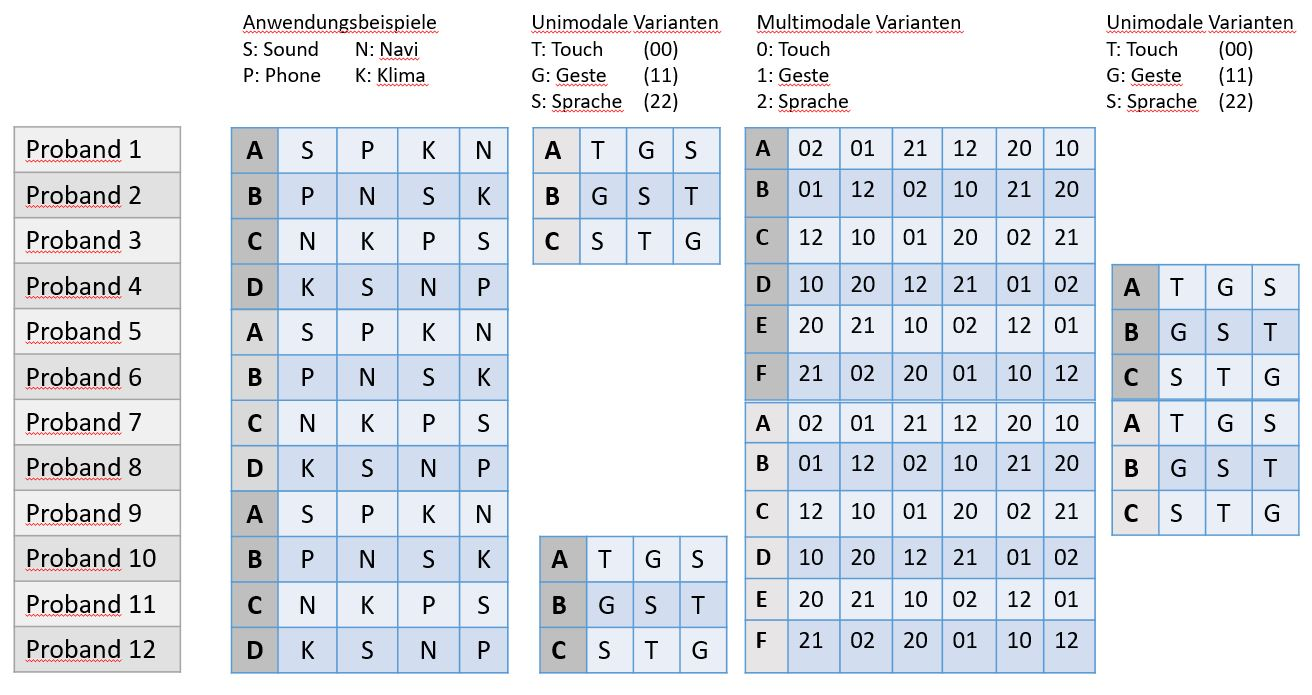
\includegraphics[width=1\textwidth]{img/Permutation.jpg}
  \caption[Permutation der Anwendungsbeispiel]{Permutation der Anwendungsbeispiel, der unimodalen Varianten und der multimodalen Varianten pro 12 Probanden}
  \label{fig:Permutation}
\end{figure} 

Um Lerneffekte zu vermeiden wurden die vier Anwendungsbeispiele mit dem Balanced Latin Square permutiert. 
Die drei unimodalen Kombinationen wurden mit dem Latin Square permutiert und die sechs multimodalen Kombinationen erneut mit dem Balanced Latin Square. 
Jede Permutation der Modalitäten wurde pro Proband für jedes Anwendungsbeispiel gleich angewendet. 

Beim Anwendungsbeispiel Navigation fielen die Varianten mit Gestik als zweite Modalität weg. 
Bei 12 Probanden ist es möglich die vier verschiedenen Permutationen der Anwendungsbeispiele drei mal zu wiederholen. 
Die drei unimodalen Kombinationen werden vier mal wiederholt und die sechs Permutationen der multimodalen Kombinationen werden zwei mal innerhalb von 12 Probanden wiederholt. 
Zudem wird die Reihenfolge von unimodalen und multimodalen abgewechselt siehe \fref{fig:Permutation}. 
Dieses Vorgehen wird für die nächsten 12 Probanden wiederholt. 
Die drei verschiedenen Zieleingaben werden ebenfalls mit dem Latin Square permutiert und auf die permutierte Moduskombination verteilt. 
Mit diesen Vorkehrungen können wir davon ausgehen, dass mögliche Lerneffekte gleich verteilt sind.   
\subsection[Fragebögen]{Fragebögen der Studie}
Es wurden zwei verschiedene Fragebögen erstellt (siehe Anhang im Kapitel \ref{cha:Anahng}). 
Im ersten Fragebogen werden demografischen Angaben wie Name , Alter, Händigkeit und die Muttersprache abgefragt. 
Außerdem die bereits gesammelten Erfahrungen im Umgang mit Interaktionen durch Touch, Geste und Sprache. 
Hier wurden, auf die Frage der Nutzungshäufigkeit, vier Antwortmöglichkeiten unterschieden:
\begin{itemize}
	\item ja, benutze ich regelmäßig 
	\item ja, benutze ich gelegentlich
	\item ja, aber nur sehr wenig
	\item nein
\end{itemize}

Nach jedem durchgeführten Messdurchgang eines Anwendungsbeispiels wurde innerhalb der Unityanwendung eine Bewertung abgefragt, wie geeignet die Probanden die eben ausgeführte Aufgabe fanden und wie sehr Ihnen die Aufgabe gefallen hat. 
Mit Touch als Eingabemodalität soll eines der fünf Symbole gewählt werden siehe \fref{fig:Smileys}.
\begin{figure}
	\centering
		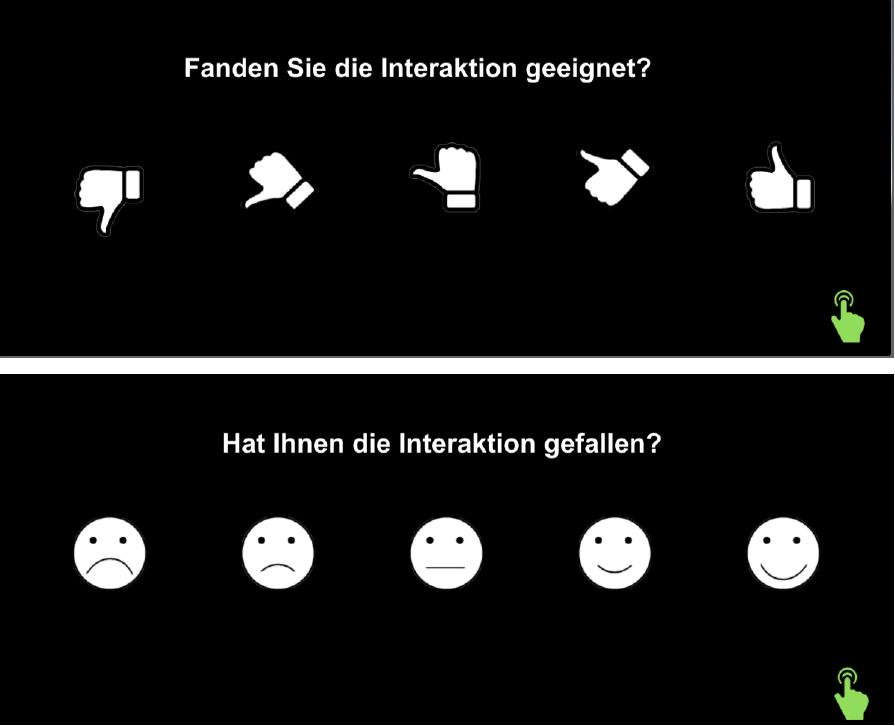
\includegraphics[width=0.7\textwidth]{img/Smileys.JPG}
	\caption[Eignung und Gefallen eines Anwendungsbeispiels]{Eignung und Gefallen eines Anwendungsbeispiels. Verwendung der Icons siehe Kapitel \ref{cha:Danksagung}.
}
	\label{fig:Smileys}
\end{figure}

Der zweite Fragebogen wird nach der Durchführung der Studie ausgefüllt. 
Darin wird abgefragt, wie geeignet die Modalitäten für die verschiedenen Screentypen sind. 
Dies wird mit einer Likertskala mit 5 Auswahlmöglichkeiten für jede Modalität abgefragt.  
Die Auswahlmöglichkeiten gehen von nicht geeignet bis geeignet. 
Außerdem wird ein Ranking für die verschiedenen Screentypen abgefragt, indem sich der Proband entscheiden muss welcher Modus für die unterschiedlichen Screentypen am besten, zweitbesten und am schlechtesten geeignet ist.  

Die kompletten Fragebögen, Einverständniserklärung, sowie der Studienleitfaden sind am Ende dieser Arbeit angehängt, siehe Kapitel \ref{cha:Anhang}.
\section{Durchführung der Studie}
Die Studie fand in Garching-Hochbrück in der Parkgarage von BMW in einem 6er Gran Coupé statt (siehe \fref{fig:GranCoupe}). 
Die Studiendauer betrug circa 1,5 Stunden. 
Das Auto wurde am Strom angeschlossen, um das Surface zu laden und eine Dauerhafte Stromversorgung für Licht sowie Sitzheizung zu ermöglichen.
\begin{figure}[ht]
  \centering
  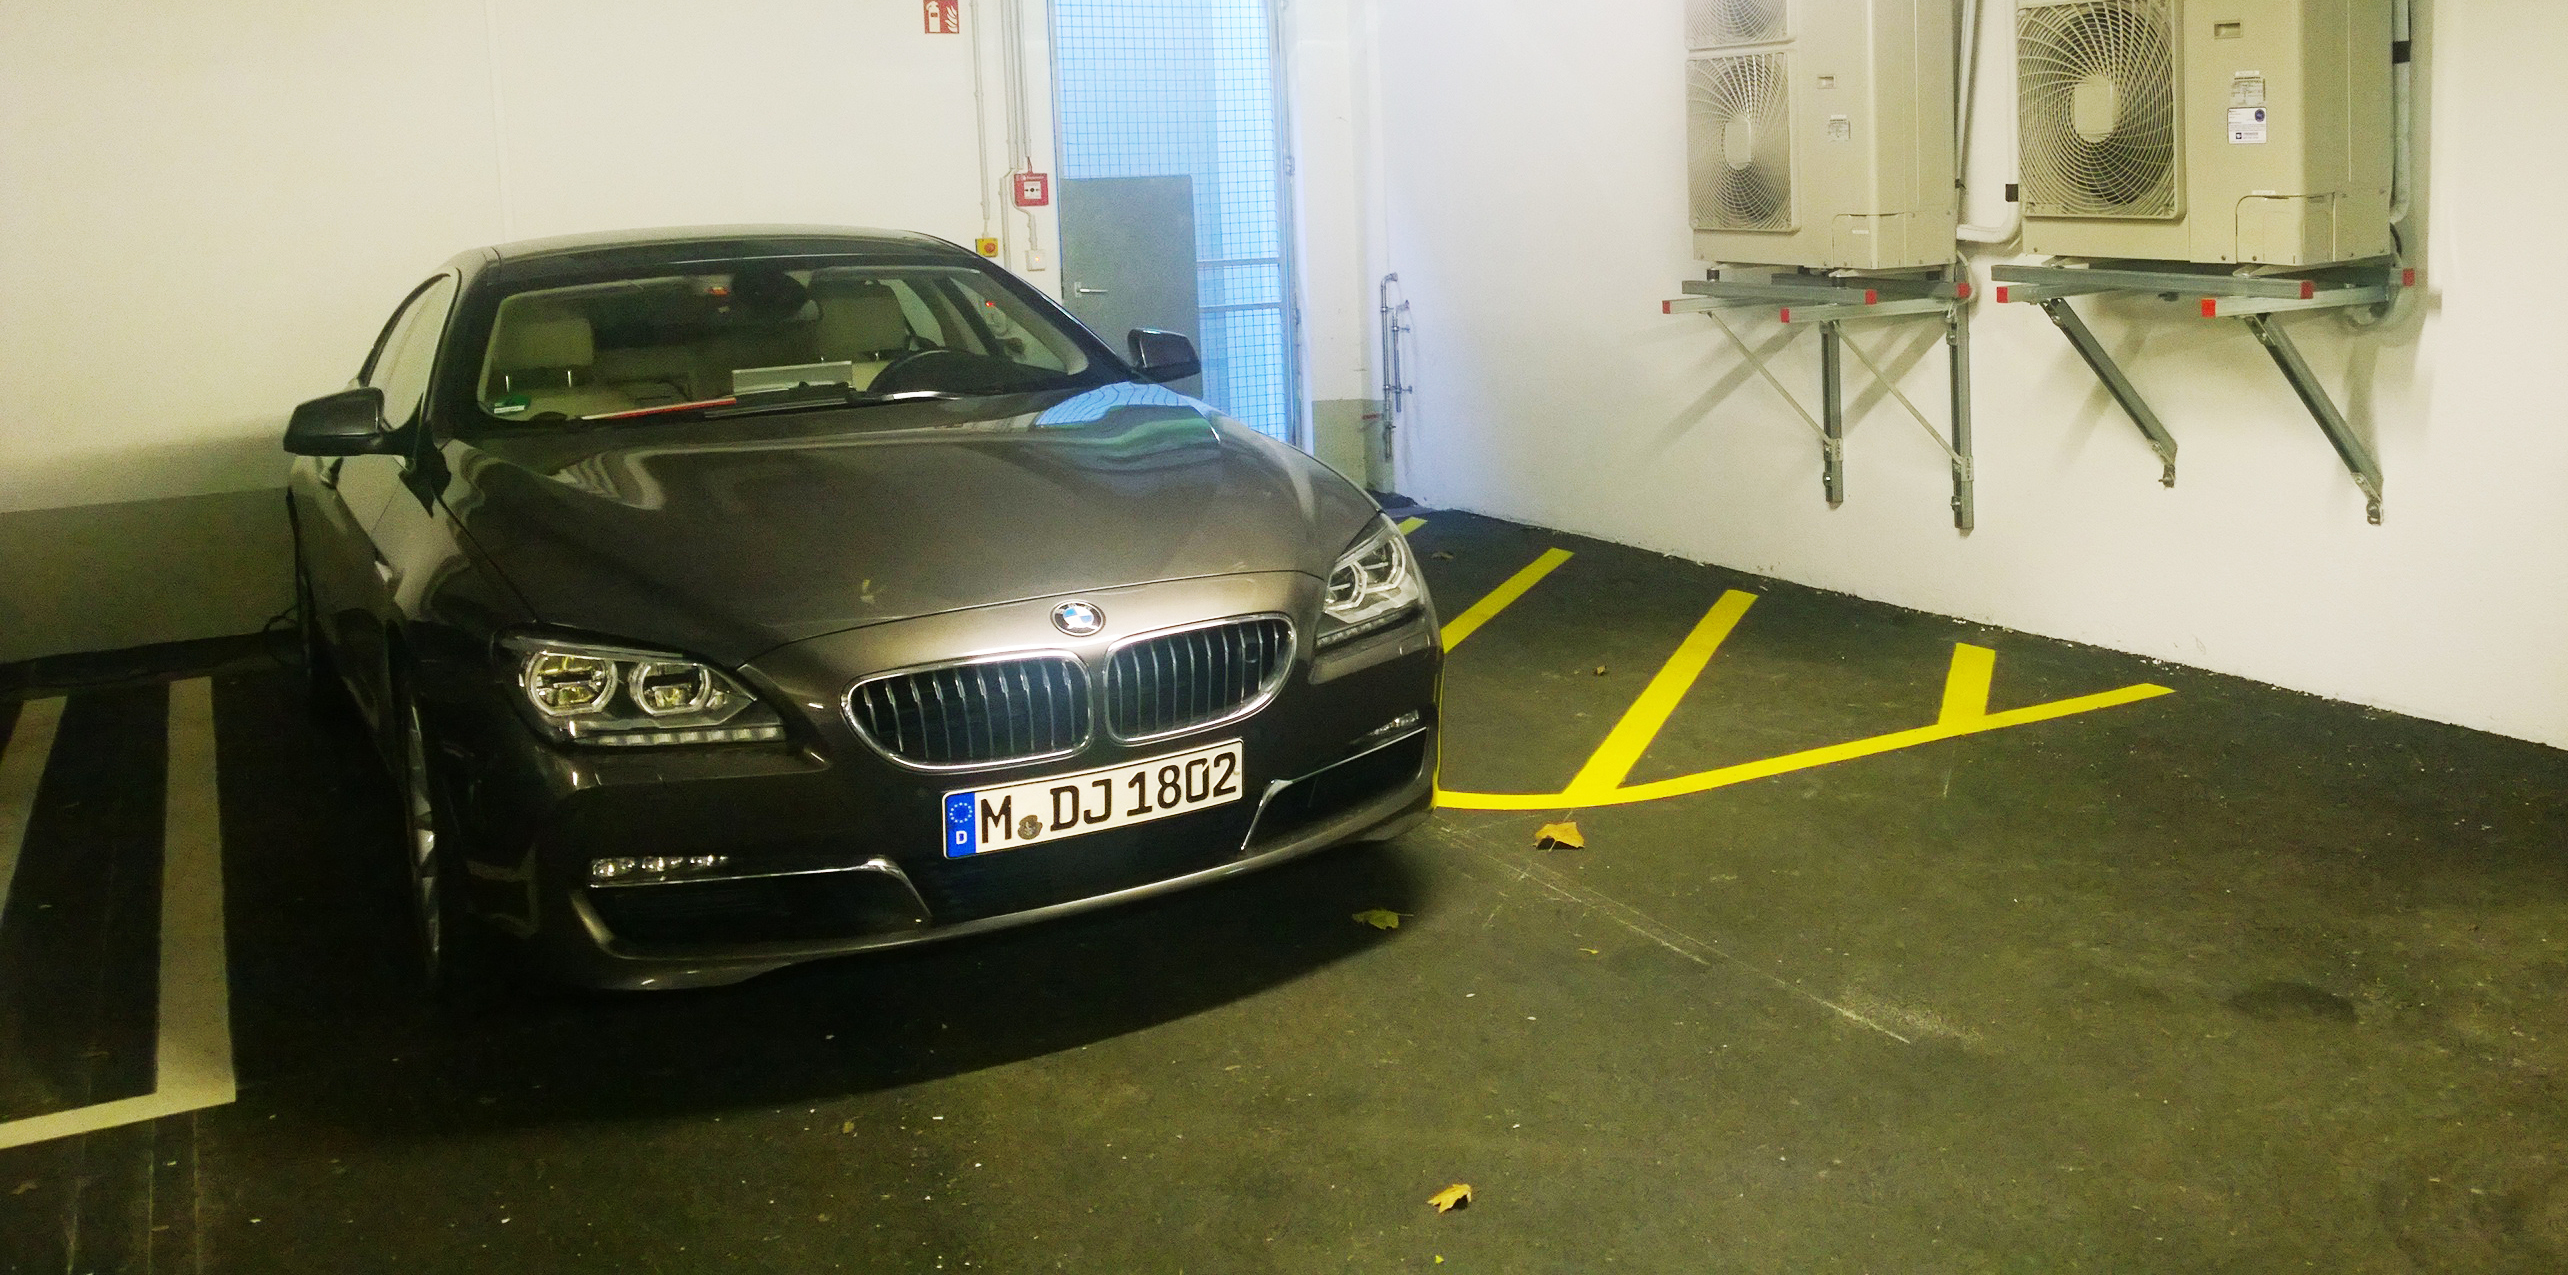
\includegraphics[width=1\textwidth]{img/GranCoupe.jpg}
  \caption{BMW 6er Gran Coupé in der Parkgarage}
  \label{fig:GranCoupe}
\end{figure} 
Das Surface wurde vor das ursprüngliche Display am Dashboard angebracht. 
Der Interaktionsbereich befand sich somit auf gleicher Höhe (siehe \fref{fig:AnbringungSurface}), jedoch etwas weiter vorne, was für den Touch auch geeigneter ist. 
Die Auflösung des Surface musste auf 1240x800 Pixel reduziert werden, damit die Darstellung groß genug war. 
Die Buttons auf dem ersten und zweiten Screen hatten somit eine Größe von 3,5 mal 4,5 cm. 

Die Leap Motion, zur Erkennung der Gesten, wurde zwischen Gangschaltung und Dashboard angebracht. 
Somit konnte die Hand bereits am Lenkrad erkannt werden, befand sich allerdings noch nicht im Interaktionsbereich, um Gesten auszuführen. 
\begin{figure}[ht]
  \centering
  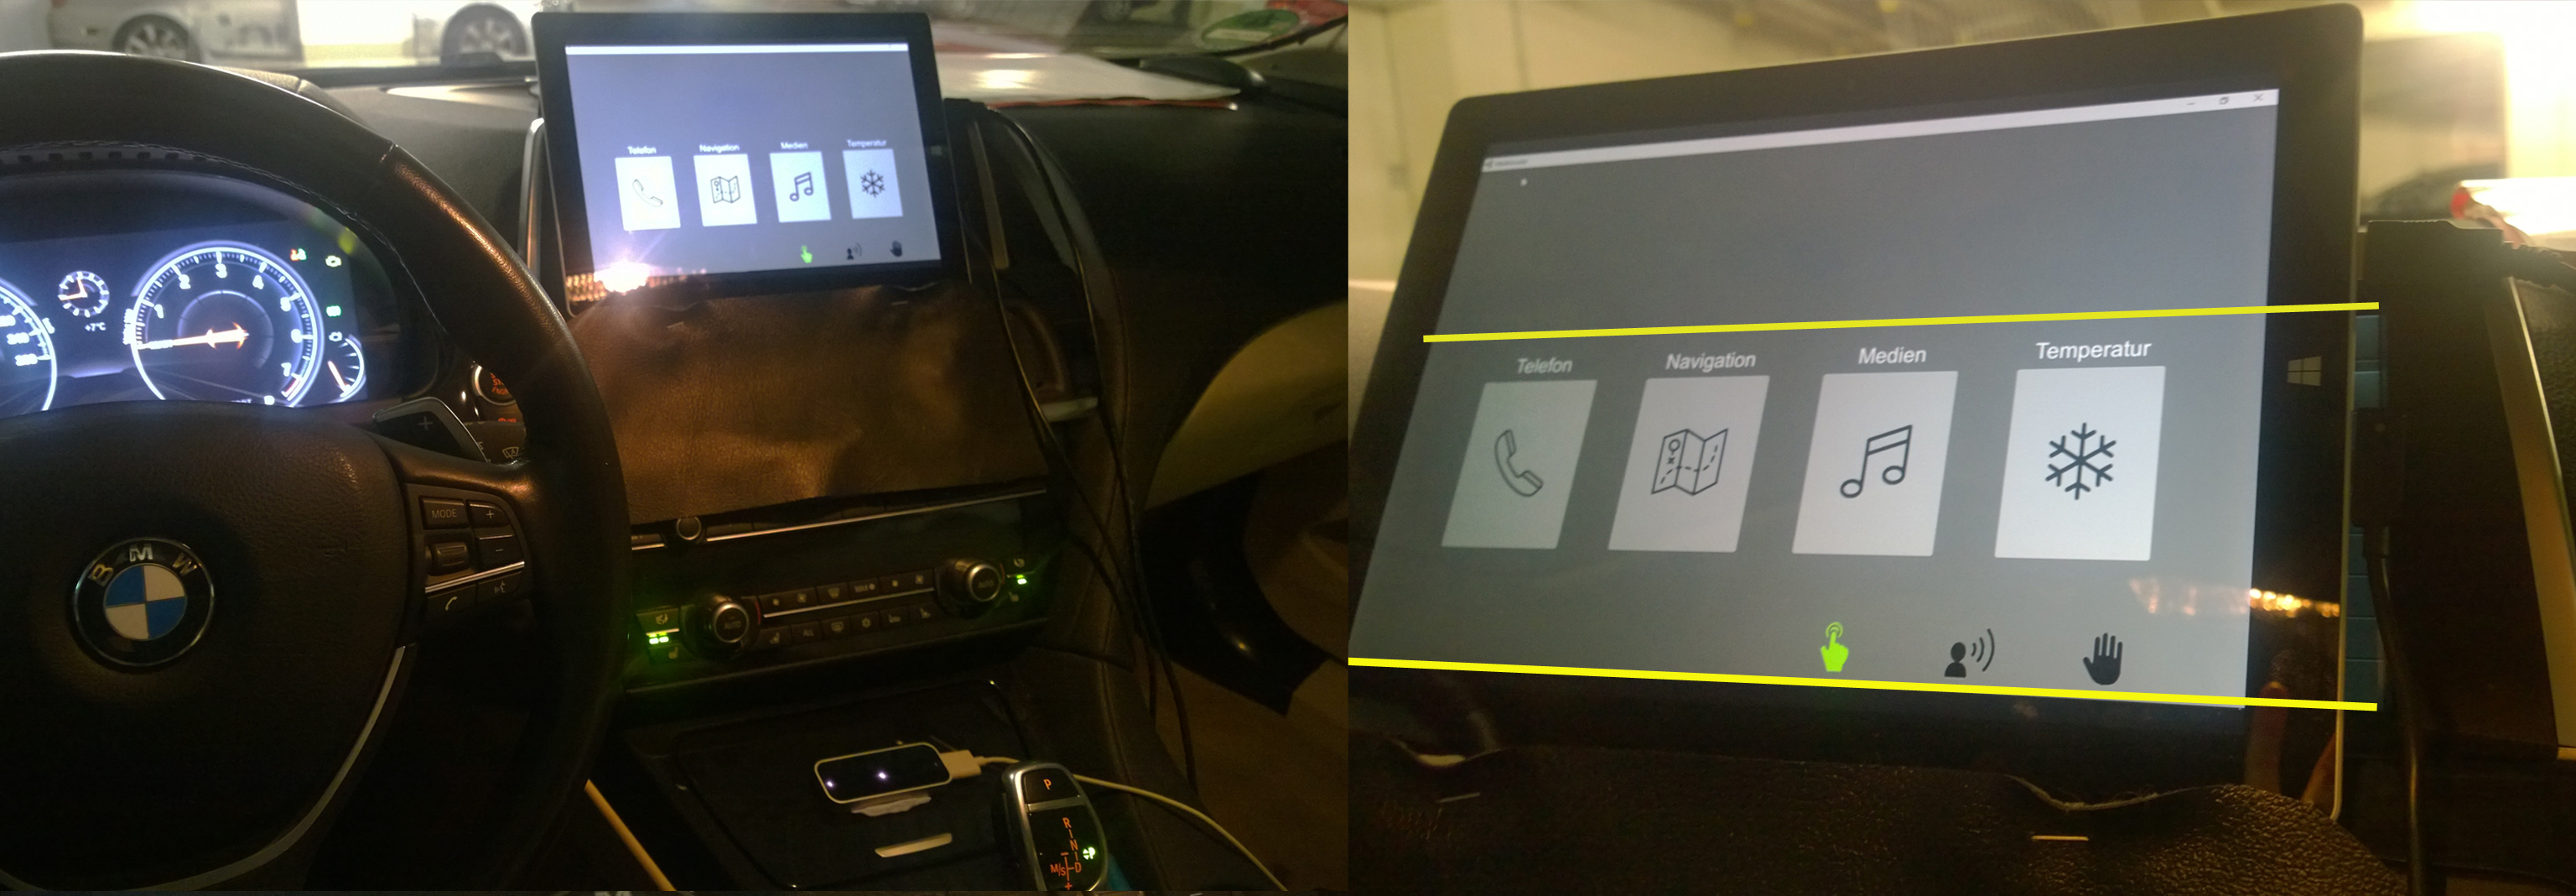
\includegraphics[width=1\textwidth]{img/AutoSetting2.jpg}
  \caption{Anbringung des Surface im Auto}
  \label{fig:AnbringungSurface}
\end{figure} 
Pro Tag konnten bis zu vier Probanden an der Studie teilnehmen. 
Bevor der erste Durchgang begann wurde das Auto am Strom über den Kofferraum angeschlossen. 
Der Akku der Go Pro wurde ausgetauscht und eine leere Speicherkarte eingelegt. 
Im Kofferraum konnten Ersatzbatterien für die Kamera geladen werden. 
Nach jedem Probanden wurde der Akku gewechselt und der gebrauchte erneut geladen. 
Die Speicherkarten von 32GB wurden immer nach zwei Probanden gewechselt und anschließend auf eine Festplatte kopiert. 
Die Kamera wurde mittig, zwischen Fahrer und Beifahrer an der Decke befestigt und Richtung Surface ausgerichtet siehe \fref{fig:Kamera}.
\begin{figure}[ht]
  \centering
  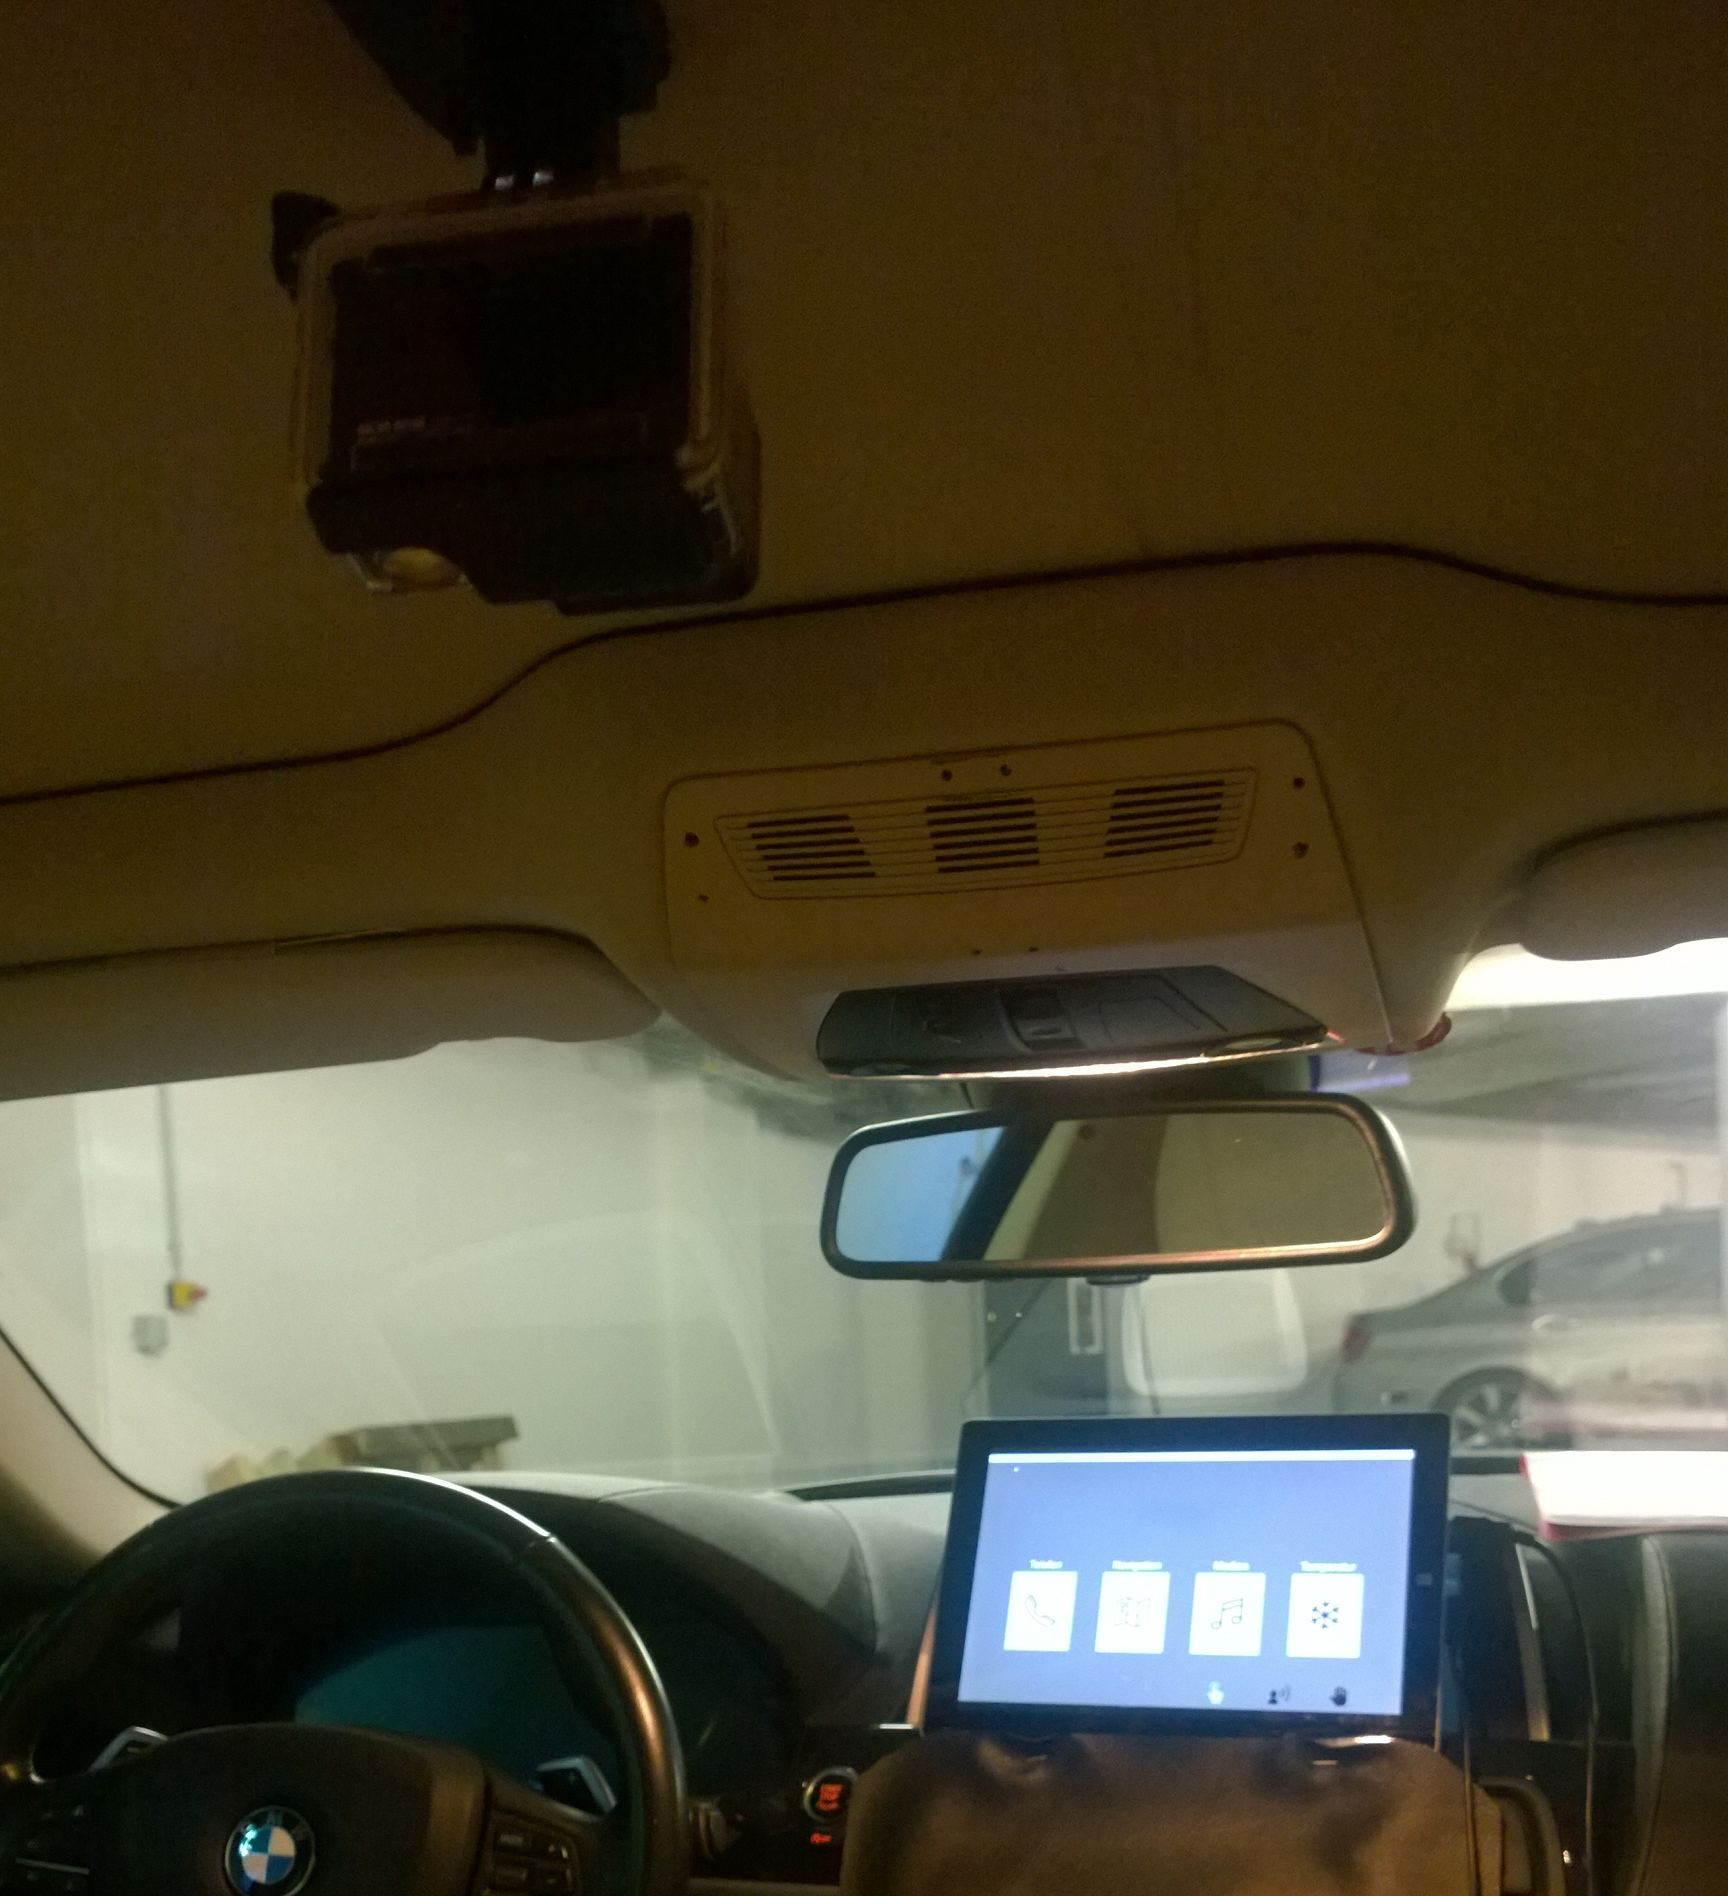
\includegraphics[width=0.5\textwidth]{img/Kamera3.jpg}
  \caption{Anbringung der Kamera im Studienauto}
  \label{fig:Kamera}
\end{figure} 

Das Surface wurde wie oben beschrieben angebracht und die Leap, sowie die externe Tastatur über einen Hub angeschlossen. 
Der Verteiler war ebenfalls an den Strom angeschlossen und wurde auf der Beifahrerseite zwischen Gurt und Mittelkonsole eingeklemmt siehe \fref{fig:Hub}. 
\begin{figure}[ht]
  \centering
  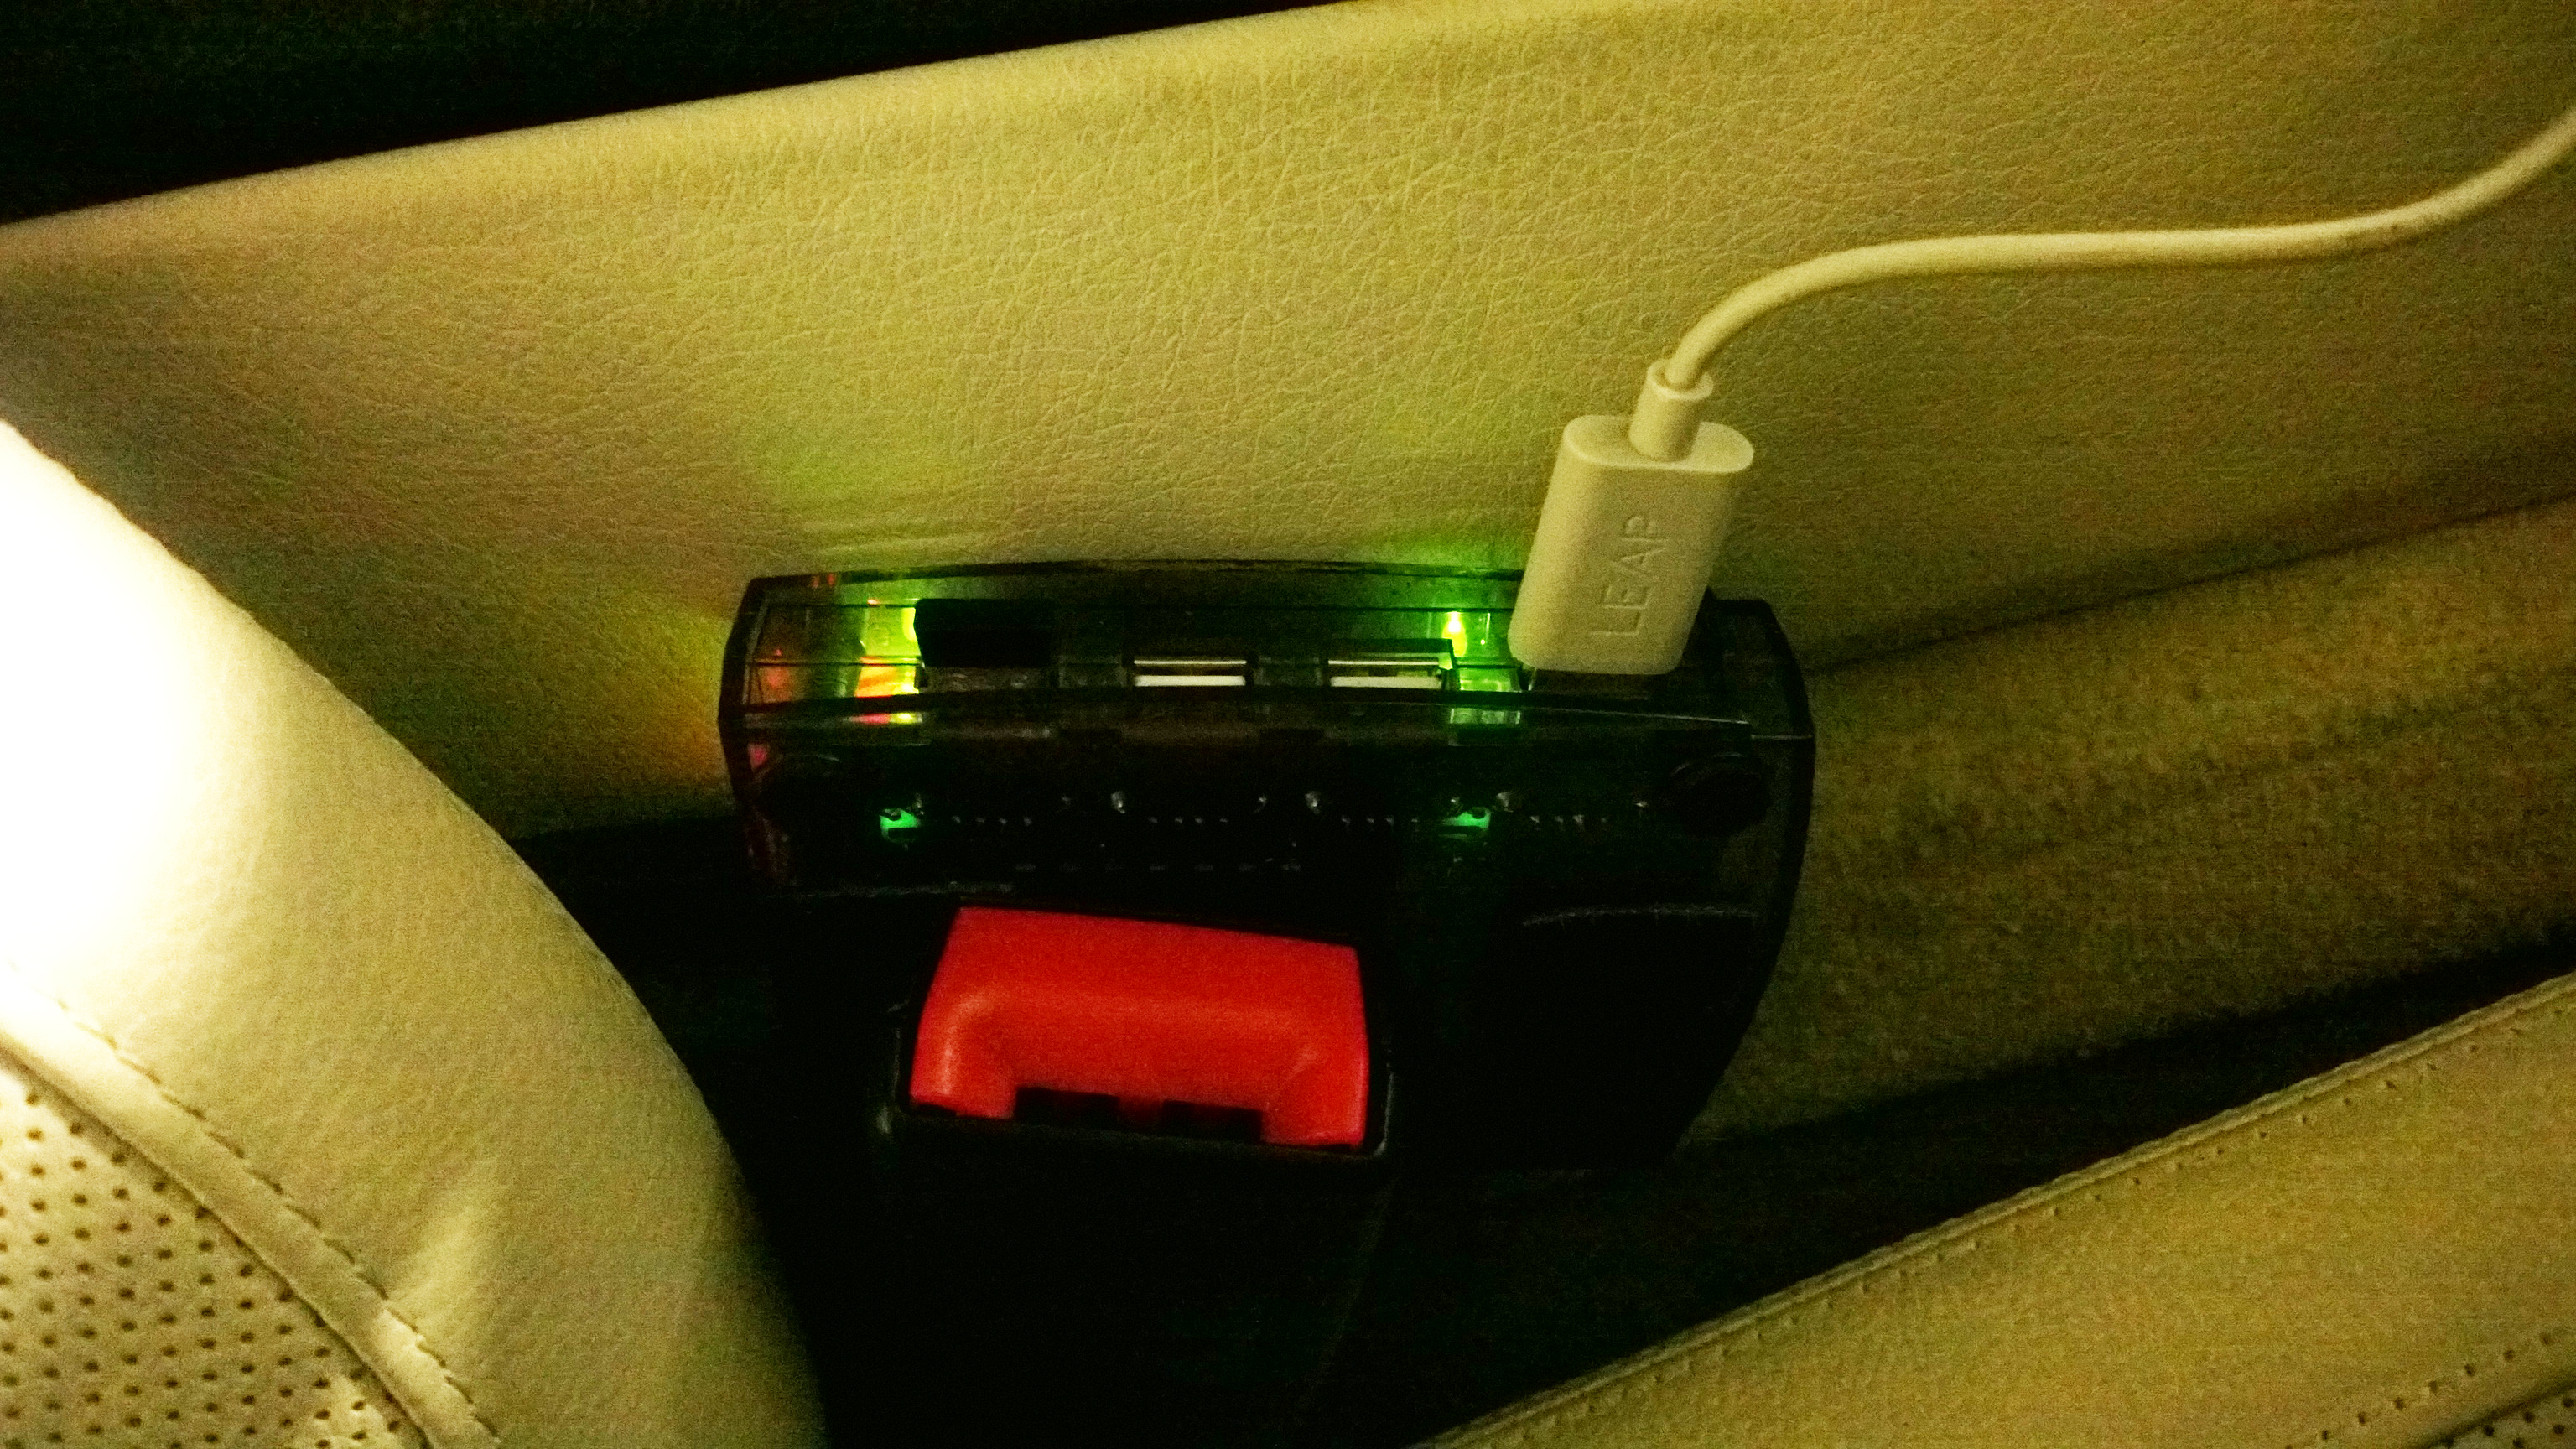
\includegraphics[width=0.5\textwidth]{img/Hub.jpg}
  \caption{Anschluss für die Leap Motion und der externen Tastatur}
  \label{fig:Hub}
\end{figure} 

Jeder Proband wurde am Empfang bei BMW am Parkrings 19 abgeholt und begrüßt.
Es wurde darauf hingewiesen, dass die Studie bis zu 1,5 Stunden dauern wird und das jetzt die beste Gelegenheit wäre, um wenn nötig noch auf die Toilette zu gehen.
Anschließend begaben wir uns in die Parkgarage zum Testfahrzeug, indem der Proband auf dem Fahrersitz platz nehmen sollte, während der Studienleiter am Beifahrersitz platz nahm.
Der Proband wurde darauf hingewiesen seinen Sitz einzustellen, als würde er oder sie das Auto fahren.

Nachdem sichergestellt wurde, dass alle Smartphones auf lautlos gestellt sind, wurde das Thema kurz erläutert und darauf aufmerksam gemacht, dass zur Erhebung der Interaktionszeiten verschiedene Daten protokolliert werden und zusätzlich die Studie mit einer Go Pro aufgezeichnet wird.

Darüber aufgeklärt musste jeder Proband eine Einverständniserklärung unterschreiben \ref{cha:Anhang}.
Zusätzlich sollte ein kurzer Fragebogen zu demografischen Daten und den Vorerfahrungen zum Umgang mit den Interaktionen Touch, Geste und Sprache ausgefüllt werden.

In der Zwischenzeit startete der Studienleiter das Programm, stellte die richtige ID ein und überprüfte die neu geladene Permutation.
Jetzt wurde das Vorgehen der Studie anhand des ersten Anwendungsbeispiel mit Hilfe der ausgedruckten Übersicht der Anwendungsbeispiele \ref{fig:UseCases} erläutert.

Sobald das erste Anwendungsbeispiel und die Vorgehensweise klar war, wurde die Go Pro gestartet und der Proband konnte mit dem ersten Probedurchlauf beginnen. Dazu hatte der Proband seine Hände am Lenkrad und der Studienleiter startete die Anwendung mit seiner externen Tastatur. 
Der Screen wird nach dem Start zuerst für 3 Sekunden schwarz bis dann der Hauptscreen zu sehen ist und die Interaktion beginnen kann.
Insgesamt gibt es 33 verschiedene Durchläufe, die jeder Proband testen soll.
Zu jedem dieser Varianten, bestehend aus den 4 Anwendungsbeispielen und deren Moduskombinationen, sollte mindestens ein Probedurchlauf gemacht werden.

Der Probedurchlauf dient dazu den Probanden mit der Aufgabe vertraut zu machen und sich an die möglicherweise neue Interaktionsmethode zu gewöhnen.
Die Probedurchläufe wurden so oft wiederholt, bis der Studienleiter das Gefühl hatte, dass die Aufgabe klar verstanden wurde. 

Nach dem Probedurchlauf werden zwei Messdurchgänge durchlaufen, die für die Erhebung der Interaktionszeiten verwendet wird.
Da wir nur fehlerfreie Messdurchgänge benötigen, wurde im Falle eines Fehlers in einem Messdurchgang, dieser wiederholt.
Passierte dies kennzeichnete der Studienleiter dies in seinen Notizen zu dieser Variante, um später nur die gültigen Messdurchgänge zu verwenden.
Auch interessante Anmerkungen oder Auffälligkeiten wurden während der Studie notiert.

Nach den mindestens 99 Durchgängen $((1 * \text{Probedurchgang} + 2 * \text{Messdurchgänge}) * 33 \text{Varianten})$ konnte die Kamera gestoppt werden und die Probanden sollten den anschließenden Fragebogen ausfüllen.
Währenddessen konnten Anmerkungen vom Versuchsleiter notiert werden. 
Als Dankeschön bekamen die Probanden nach der Studie Schokolade.

Nach jedem Studiendurchgang wurde der Akku der Kamera gewechselt. Die Speicherkarte wurde nach jedem zweiten Probanden gewechselt.
\section[Quantitative Auswertung]{Quantitative Auswertung der Studienergebnisse}
Im folgenden werden die quantitativen Ergebnisse der Studie präsentiert.
In einem Zeitraum von 2 Wochen nahmen insgesamt 22 Probanden an der Studie zur Erhebung der Interaktionszeiten teil.
hierbei wurden über 22 Stunden Videomaterial aufgezeichnet. 
\subsection[Studienteilnehmer]{Studienteilnehmer}
Das Alter der 22 Studienteilnehmer (14 männlich und 8 weiblich) beträgt im Durchschnitt 30,55 Jahre. 
Der Altersbereich erstreckt sich von 22 bis 58 Jahren. 
Mode und Median ergaben je 25 Jahre. 19 der 22 Probanden sind rechtshändig, 2 linkshändig und ein Proband gab an beidhändig zu sein. 
Alle Teilnehmer sprechen deutsch als Muttersprache.

Die Vorerfahrungen mit der Bedienung von Touch, Gesten und Sprache der Teilnehmer wurde von den Probanden abgefragt und von den Probanden eingeschätzt. 
Auf die Frage, ob sie Erfahrung mit der Bedienung von Sprache, Touch und Geste haben, konnte aus vier Optionen gewählt werden (1: nein, 2: ja, aber nur sehr wenig, 3: ja, benutze ich gelegentlich und 4: ja, benutze ich regelmäßig). 

Die Vorerfahrung von Sprache ergab im Durchschnitt 2,32, bei Touch 3,95 und bei Geste 1,86. Die genauen Angaben der Probanden können aus \fref{fig:Vorerfahrung} entnommen werden.
\begin{figure}[ht]
  \centering
  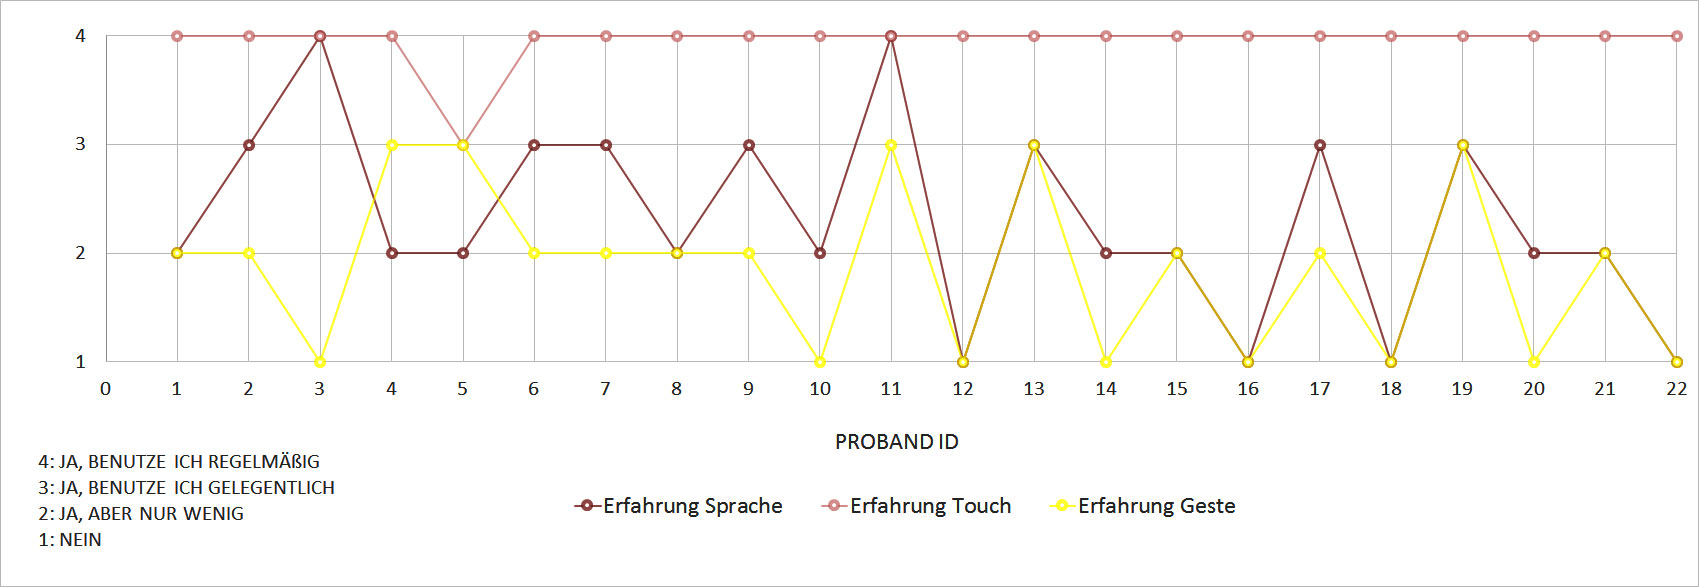
\includegraphics[width=1\textwidth]{img/ErfahrungProbanden2.jpg}
  \caption[Vorerfahrung der Probanden]{Vorerfahrung der Probanden mit der Bedienung von Touch, Sprache und Geste. Einschätzung der Probanden auf die Frage: Haben Sie Erfahrung bei der Bedienung von Sprach-, Touch- und Gestensteuerung.}
  \label{fig:Vorerfahrung}
\end{figure} 
\subsection[User Experience]{User Experience}
Nach jedem Messdurchgang wurden die Nutzer gefragt wie geeignet Sie diese Interaktion fanden und, ob sie Ihnen gefallen hat. 
Wie bei einer Likert-Skala werden 5 Antwortoptionen unterschieden. Zwei negative, eine neutrale und zwei positive (siehe \fref{fig:Uebersicht_Eignung}). 
Aus den Antworten ist deutlich zu sehen, dass die unimodale Variante mit Sprache in beiden Bereichen immer am besten abschnitt. 
Die Unterschiede zwischen Eignung und Gefallen sind nicht sehr groß, allerdings fällt auf, dass vor allem die Interaktionen mit Geste den Nutzern besser gefällt als sie deren Eignung einschätzen. 
Am zweit beliebtesten in beiden Kategorien war die Kombination von Touch und Sprache. 
Bei dem Anwendungsbeispiel Lautstärke war die Kombination Touch und Sprache sogar in Eignung und Gefallen noch etwas besser als die unimodale Sprachvariante. 
Die dritt beliebteste Variante vom Lautstärkebeispiel war die Kombination Sprache und Touch. 
Bei allen anderen Anwendungsbeispielen war die dritt beliebteste Kombination Geste und Sprache. 

Grundsätzlich lässt sich sagen, dass die Mehrheit der Probanden die Sprache am geeignetsten empfanden. Nur für die Direktauswahl aus sichtbaren Elementen schnitt Touch etwas besser ab als Sprache. 
Die Geste hat bei der Direktauswahl die besten Ergebnisse verglichen zu den anderen Operatoren. 
Ein sehr eindeutiges Ergebnis aus den Fragebögen bekommen wir bei der Texteingabe, die eindeutig für Sprache besser geeignet ist, als per Touch das gewünschte Ziel einzutippen siehe \fref{fig:Uebersicht_Eignung}.
\begin{figure}[ht]
  \centering
  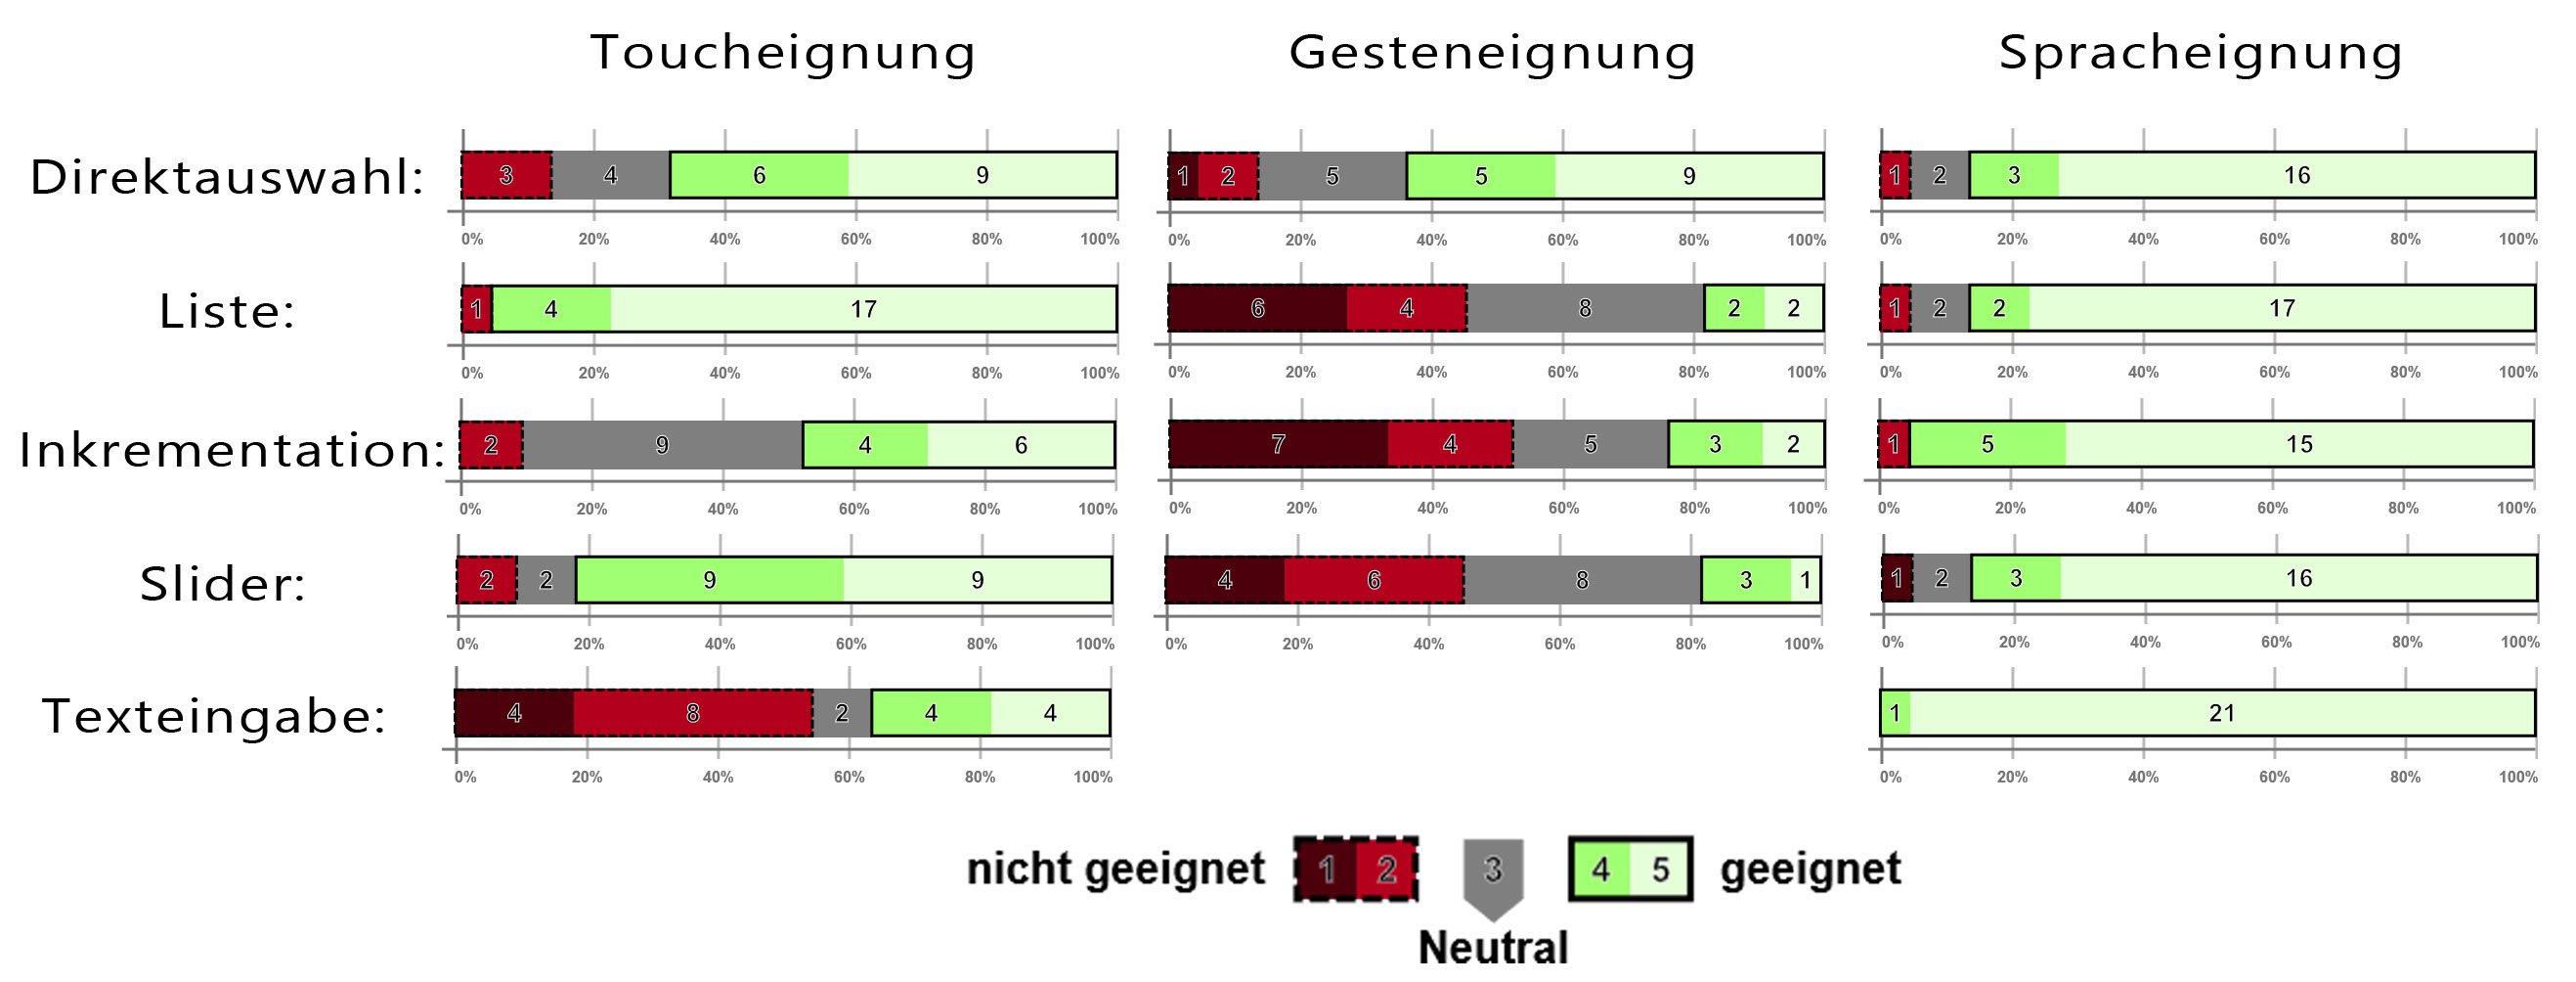
\includegraphics[width=1\textwidth]{img/Uebersicht_Eignung}
  \caption[Eignung des Screentypen]{Einschätzung der Probanden, wie geeignet Sie die verschiedenen Screentypen für die jeweilige Modalität halten. 
	Die Balkendiagramme zur Darstellung von Likert-Skalen wurde mit http://likertplot.com/ generiert.}
  \label{fig:Uebersicht_Eignung}
\end{figure}

Im zweiten Teil des Fragebogen sollten die Screentypen noch mit einem Ranking bewertet werden. 
Hier mussten sich die Probanden entscheiden welche Modalität am besten, zweitbesten und am schlechtesten geeignet ist. 
Bei der Direktauswahl aus sichtbaren Elementen halten 10 von 22 die Toucheingabe, 8 die Sprachbedienung und 4 die Gestensteuerung am geeignetsten. 
Bei den restlichen Screentypen wird die Sprachbedienung am häufigsten für am geeignetsten gehalten. 
Sehr eindeutig sind die Ergebnisse der Texteingabe. 
21 von 22 Probanden finden die Spracheingabe für Texteingaben geeigneter, als das Ziel Buchstabe für Buchstabe einzutippen.

\subsection[Ermittlung der Zeiten der Aktionen]{Ermittlung aller Zeiten der Aktionen}
Um die Zeiten der Operatoren zu ermitteln werden die Differenzen zwischen den gewünschten protokollierten Events berechnet. 
Dafür musste zuerst unsere Protokollierung etwas aufbereitet werden. 
Als erstes wurde die Logdatei in eine Excelltabelle in Tabellenformat geladen. 
Somit können für die Auswertung nach beliebigen Kriterien die Spalten gefiltert und sortiert werden. 

Fehlerhafte Messdurchgänge wurden, anhand der Notizen während der Studie, als fehlerhaft markiert. 
In einigen wenigen Fällen gab es bei manchen Kombinationen drei statt zwei Messdurchgängen. 
Hier wurde der dritte Durchgang immer behalten und von den ersten beiden der schlechteste verworfen. 
Bei Unklarheiten konnte das Videomaterial zur Überprüfung hinzugezogen werden, bis es zu jedem Probanden zwei fehlerfreie Messdurchgänge in jeder Kombination gab. 

Für die Berechnungen der verschiedenen Zeiten wurden die protokollierten Events verwendet. 
Ein Beispiel dafür wäre die Zeit, die ein Nutzer benötigt, bis der erste Button gedrückt wird (DA des ersten Screens). Als Startzeit wurde die protokollierte Zeit vom Event "`MainUI"' benutzt. 
Der Screen des Hauptmenüs heißt MainUI. Da unsere Interaktion begann, sobald der Hauptscreen zu sehen war, entspricht das Laden dieser Szene unserem Startpunkt. 
Dafür wurde eine neue Spalte der Excelltabelle angelegt und immer wenn das protokollierte Event "`MainUI"' in der Spalte "`Szenen"' gefunden wird, wird die protokollierte Zeit aus der Spalte "`ms Gesamt"' in die neue Spalte geschrieben. 
Wenn die Bedingung nicht erfüllt ist, wird der Wert der Zelle darüber in die Zelle geschrieben. 
Gibt man folgende Formel in die Spalte ein wird sie automatisch in der kompletten Spalte berechnet.  
\begin{lstlisting}
=IF([@Szenen]="MainUI";[@[ms Gesamt]];AJ59)
\end{lstlisting}
Das Ende der Aktion ist das Event "`Button geklickt: (Name der 4 Buttons)"'. 
Dafür wurden alle vier Buttons (Telefon, Navigation, Medien und Temperatur) des Hauptscreens verwendet. 
Um daraus jetzt die Dauer einer Aktion zu berechnen wurde die Differenz der Zeitpunkte berechnet und durch 1000 geteilt um die Zeit in Sekunden zu bekommen.
\begin{lstlisting}
=IF([@[Endzeit Spalte]]-[@[Startzeit Spalte]]>0;
([@[Endzeit Spalte]]-[@[Startzeit Spalte]])/1000;0)
\end{lstlisting}

Mit Berechnungen dieser Art wurden alle Zeiten ermittelt. Die Tabelle kann nach Anwendungsbeispiel, Moduskombination und Event sortiert werden, um die gewünschten Zeiten für die Auswertung zu verwendet. 
Anzumerken ist, dass diese Art der Berechnung auch Antwortzeiten des Systems beinhalten. 
Wir werden uns relevante Größen separat anschauen, um diese später als konstanten Wert im Modell zu berücksichtigen. 
Zum Beispiel haben wir eine Animation einer scrollenden Liste eingebaut, um dem Nutzer ein besseres Feedback zu gewährleisten. 
Diese Animationszeit wird separat als Antwortzeit unseres Prototypen betrachtet. 

Im folgenden schauen wir uns die Ergebnisse der Studie an. 
Wir gehen in diesem Abschnitt noch nicht auf Signifikante Unterschiede ein, sondern schauen uns zunächst die Ergebnisse und deren Auffälligkeiten näher an. 

Die ersten beiden Screens für die Anwendungsbeispiele Telefon, Navigation und Medien und der erste Screen für das Anwendungsbeispiel Temperatur, bestehen je aus einer Direktauswahl aus sichtbaren Elementen (DA). 
Der Startpunkt der Berechnung war das Laden des Hauptmenüs. 
Die Nutzer wurden angewiesen mit der Interaktion zu beginnen, sobald sie den Hauptscreen sehen. 
Das Ende der Direktauswahl aus sichtbaren Elementen war das protokollierte Event das der Button geklickt wurde. 
Je nach Anwendungsbeispiel (Telefon, Navigation, Medien und Temperatur) musste ein anderer Button selektiert werden. 
Es wurden alle 4 verschiedene Button einmal verwendet, siehe \fref{fig:UseCases}.
\begin{figure}[ht]
  \centering
  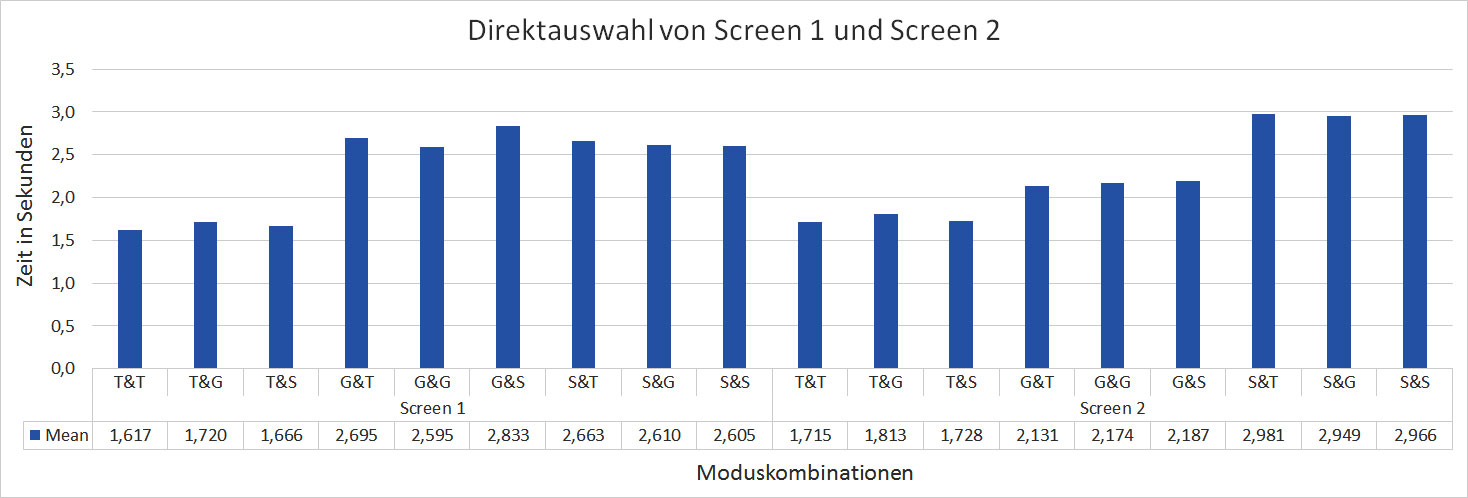
\includegraphics[width=1\textwidth]{img/DA_Screen12.JPG}
  \caption[Durchschnittszeiten in Sekunden der Direktauswahl]{Durchschnittszeiten und Medianwerten in Sekunden der Direktauswahl beider Screens für alle Moduskombinationen. T steht für Touch, S für Sprache und G für Geste.}
  \label{fig:DA_Screen12}
\end{figure}
In \fref{fig:DA_Screen12} werden die Durchschnittszeiten von allen Moduskombinationen der beiden Screens abgebildet. 
Für diese Aktion spielt jedoch nur der erste Modus eine Rolle, da der Moduswechsel erst anschließend statt findet. 
Die Auswahl der Buttons per Touch ist auf beiden Screens am schnellsten. 
Im ersten Screen liegen die Interaktionszeiten für Geste und Sprache sehr nah zusammen. 
Im zweiten Screen dauert die Spracheingabe deutlich länger als per Gestensteuerung.
Wie zu erwarten scheint der nachfolgende Modus keinen großen Einfluss auf die Interaktionszeit zu nehmen. 
Uns interessiert im speziellen der Einfluss nach einem Wechsel. 

Als nächstes stellen wir Aktionen vor, die nach einem potentiellen Moduswechsel statt finden. 
Die Modalität, die in dieser Aktion ausgeführt wird ist somit die zweite Modalität. 
Im Falle der unimodalen Variante findet kein Moduswechsel statt. 
Findet ein Moduswechsel statt, bezeichnen wir im folgenden die zusätzliche Zeit als Wechselkosten. 
Sie beinhalten einen mentalen Operator und den Homing Operator, da bei einem Moduswechsel zu Geste oder Touch die Position der Hand geändert wird.

Die erste Aktion, die wir uns nach einem Moduswechsel ansehen, ist die Aktion Listen-Navigation (L). 
Die Probanden mussten im Anwendungsbeispiel Telefon die Liste um 3 Seiten inkrementieren und schließlich den Kontakt "`Maria Müller"' durch eine Direktauswahl wählen. 
Im ersten Swipe stecken unsere Wechselkosten mit drinnen, weswegen dieser auch deutlich länger dauert, als die anderen beiden Swipes siehe \fref{fig:Swipe13Phone}. 
Der Startpunkt des ersten Swipes ist der Zeitpunkt, sobald der Screen mit der Liste geladen wurde. 
Wurde die Liste um eine Seite gescrollt, ist das der Endpunkt des ersten Swipes und gleichzeitig der Startpunkt des zweiten Swipes und genauso für den Dritten. 
\begin{figure}[ht]
  \centering
  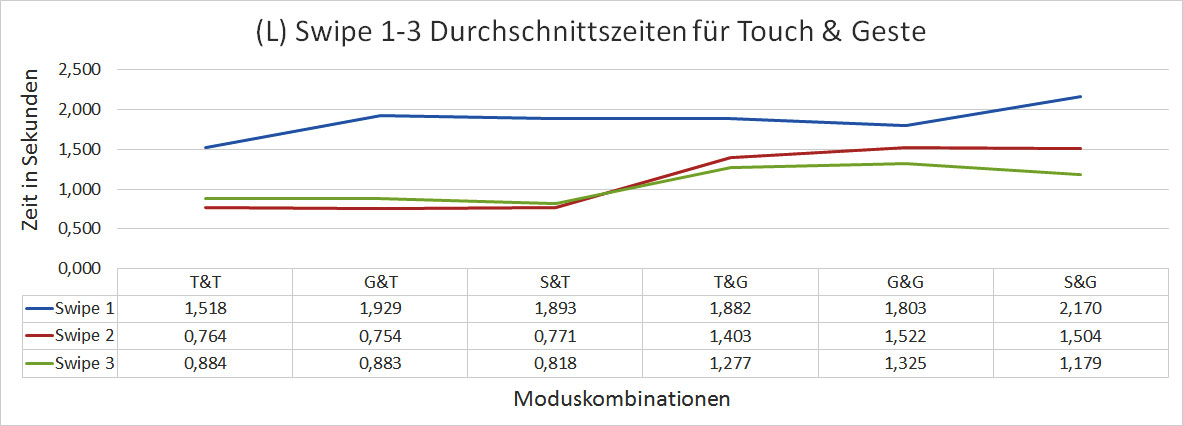
\includegraphics[width=1\textwidth]{img/Swipe1-3_Phone.JPG}
  \caption{Durchschnittszeiten für Swipe 1, 2 und 3 in Sekunden der Liste für die Moduskombinationen von Touch und Geste}
  \label{fig:Swipe13Phone}
\end{figure}
Es fällt auf, dass beim ersten Swipe die unimodalen Varianten schneller sind als die multimodalen Varianten. 
Der Wechsel einer Modalität benötigt etwas mehr Zeit, da der mentale Operator wahrscheinlich etwas länger dauert und auch die Umpositionierung der Hand wegfallen kann. 

Anschließend folgt die Aktion Direktauswahl innerhalb der Liste von "`Maria Müller"', siehe \fref{fig:DA_Swipe}. 
Es ist eine deutlich kürzere Zeit als die Direktauswahl vom ersten Screen, da sich die Hand des Nutzer bereits im richtigen Interaktionsbereich befindet. 
Daher sollten wir diese Aktion zusätzlich unterscheiden. 
Die Direktauswahl aus sichtbaren Elementen innerhalb der Liste startet unmittelbar nach dem dritten Swipe und endet mit der Selektion des Button "`Maria Müller"'.
\begin{figure}[ht]
  \centering
  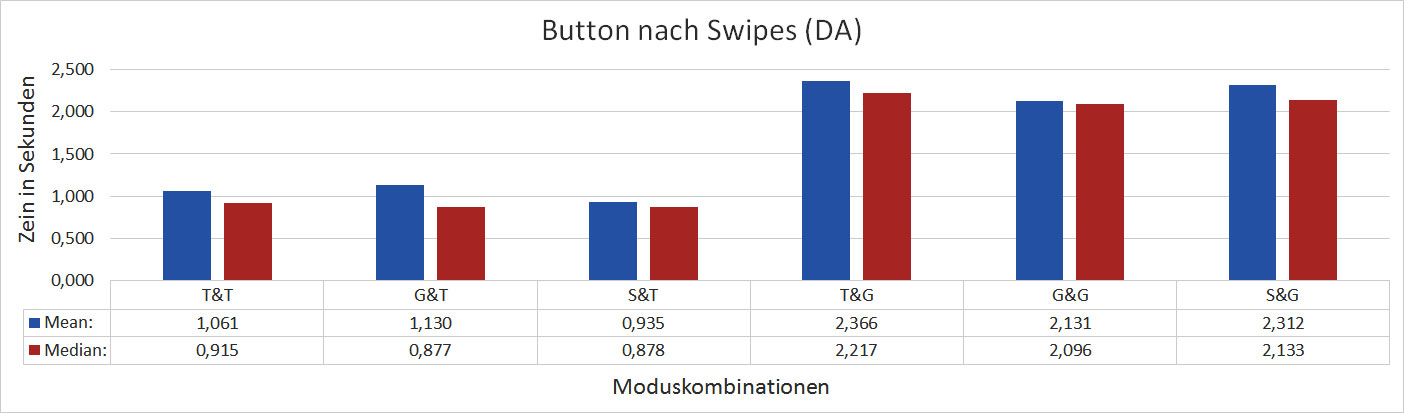
\includegraphics[width=1\textwidth]{img/DA_Swipe.JPG}
  \caption{Durchschnittszeiten in Sekunden für die Direktauswahl innerhalb der Listen Aktion}
  \label{fig:DA_Swipe}
\end{figure}

Die Touchzeiten der Texteingabe durch Buchstaben, der drei verschiedenen Ziele können aus \fref{fig:TouchzeitenB_Ges} entnommen werden. 
Es ist deutlich ein Muster zu erkennen. 
Der erste Buchstabe dauert am längsten, da hier erneut die Wechselkosten hinzukommen. 
Auch bei dieser Aktion des ersten Buchstaben ist die unimodale Variante mit 1,765 Sekunden (Touch-Touch) im Durchschnitt schneller als die Multimodalen Varianten mit 1,990 Sekunden (Geste-Touch) und 1,983 Sekunden (Sprache-Touch).
Der zweite und dritte Buchstabe ist schon deutlich schneller und alle weiteren Buchstaben nähern sich dem Wert einer halben Sekunde an. 
Der Start der Texteingabe beginnt wieder mit dem laden der Szene des Texteingabescreens. Jeder Buttonklick eines Buchstaben ist die Endzeit des vorherigen Buchstaben und die Startzeit des nächsten Buchstabens.
\begin{figure}[ht]
  \centering
  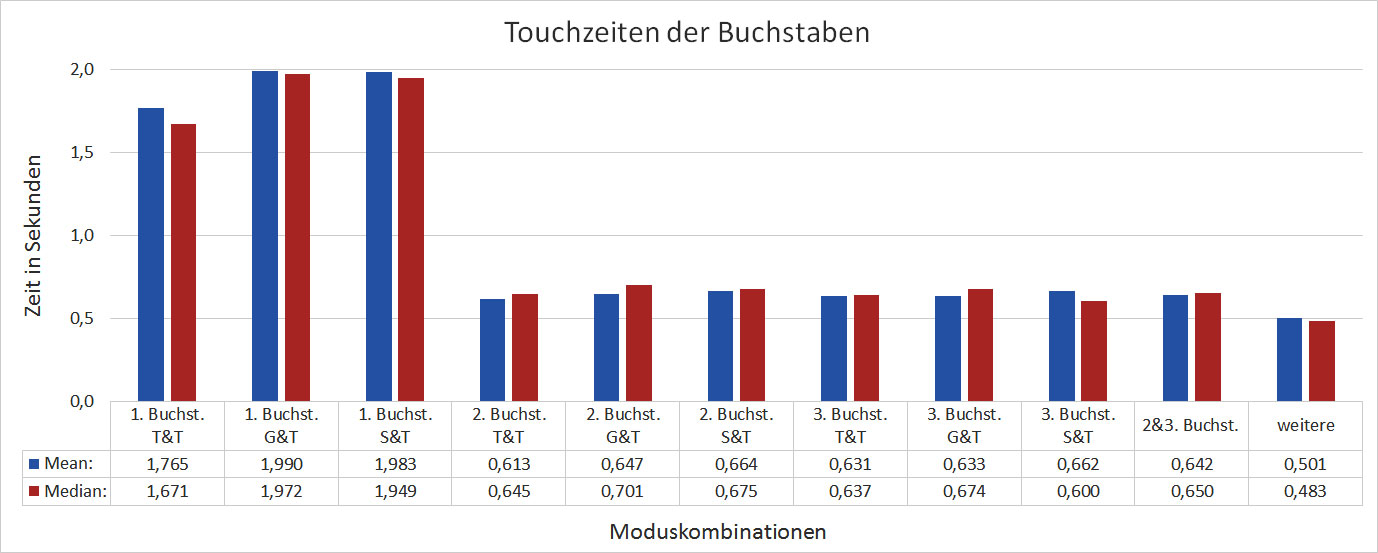
\includegraphics[width=1\textwidth]{img/TouchzeitenBuchstabenGesamt.jpg}
  \caption{Durchschnittszeiten für Touch in Sekunden der einzelenen Buchstaben}
  \label{fig:TouchzeitenB_Ges}
\end{figure}
\begin{figure}[ht]
  \centering
  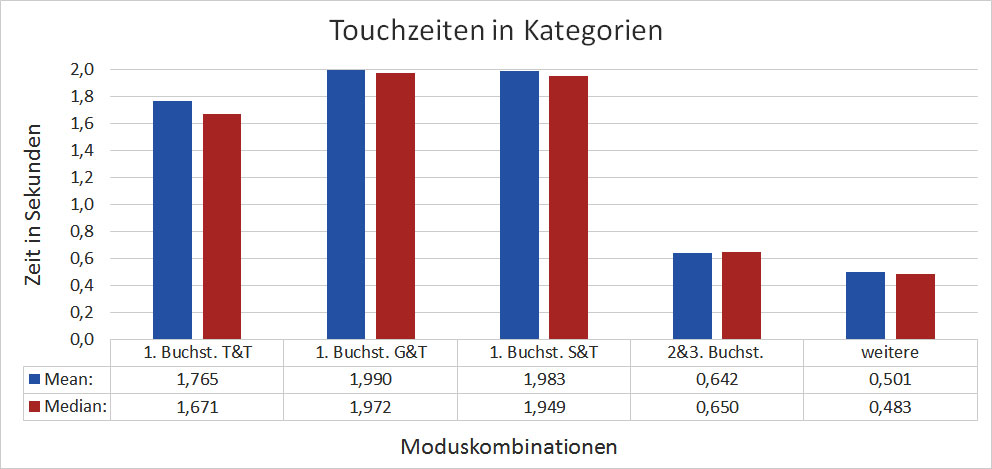
\includegraphics[width=1\textwidth]{img/TouchzeitenKategorien.JPG}
  \caption[Kategorien der Buchstaben für Wörter.]{Kategorien der Buchstaben für Wörter. Hier wurden von den drei verschienenen Zielen (Rom, Dirfweg und Kirchngasse) jeweils die ersten, zweiten und dritten und alle weiteren Buchstaben zusammengefasst.}
  \label{fig:Kategorien}
\end{figure} 

In \ref{fig:TouchzeitenB_Ges} kann man deutlich erkennen, dass sich der zweite und dritte Buchstaben nicht deutlich unterscheiden und die restlichen Buchstaben nochmals schneller eingegeben wurden. 
Wir haben deshalb entschlossen beim ersten Buchstaben den vorherigen Modus zu unterscheiden. 
Den zweiten und dritten Buchstaben zusammenzufassen und für alle weiteren Buchstaben den Durchschnitt dieser zu verwenden. 
Wir kommen somit auf 3 Kategorien. Der erste Buchstabe mit Unterscheidung der vorherigen Modalität, eine gemeinsame Zeit für den zweiten und dritten Buchstaben und als letztes, eine Zeit für alle weiteren Buchstaben \ref{fig:Kategorien}.

Bei der Sprache ist das Ergebnis weniger deutlich (siehe \ref{fig:SpracheZiel}). 
Was allerdings klar zu erkennen ist, dass Rom immer am schnellsten war. 
Bei Dorfweg und Kirchengasse ist es nicht so eindeutig. 
Auch hier ist das Laden der Szene der Startpunkt und das Ende ist das Event, indem das Inputfeld mit dem Ziel gefüllt wird.
\begin{figure}[ht]
  \centering
  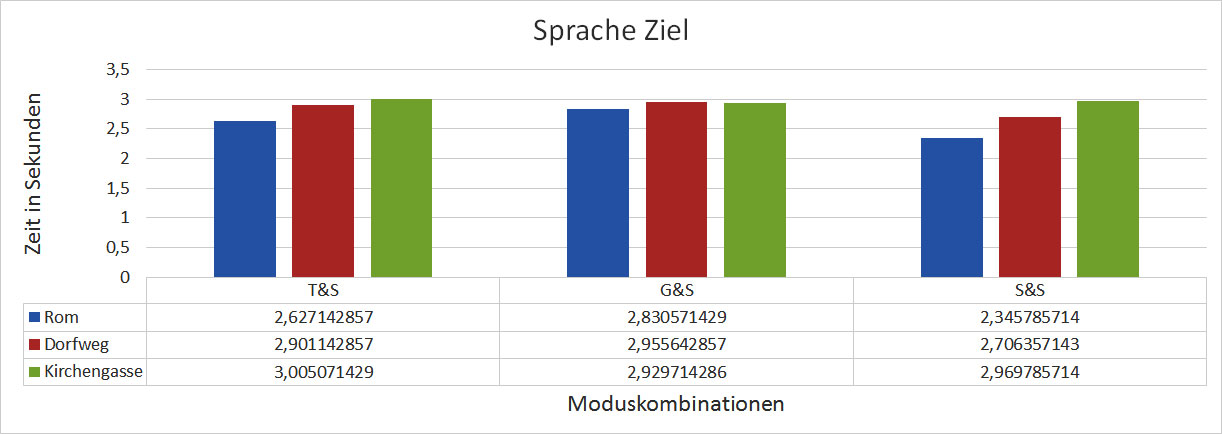
\includegraphics[width=1\textwidth]{img/SpracheZiel.JPG}
  \caption{Durchschnittszeiten in Sekunden der Ziele für Sprache}
  \label{fig:SpracheZiel}
\end{figure} 

Nach dem Touch und den Spracheingaben der Ziele wird noch die Bestätigung des OK Buttons gemessen. 
Die Aktion startet mit dem letzten Buchstaben der Toucheingabe oder dem Aktualisieren des Inputfeld der Spracheingabe. 
Der Moduswechsel fand bereits statt und wie zu erwarten sind die Abweichungen zum vorherigen Modus sowohl bei Touch, als auch bei der Spracheingabe sehr gering (siehe \ref{fig:Bestaetigung_OK}).
\begin{figure}[ht]
  \centering
  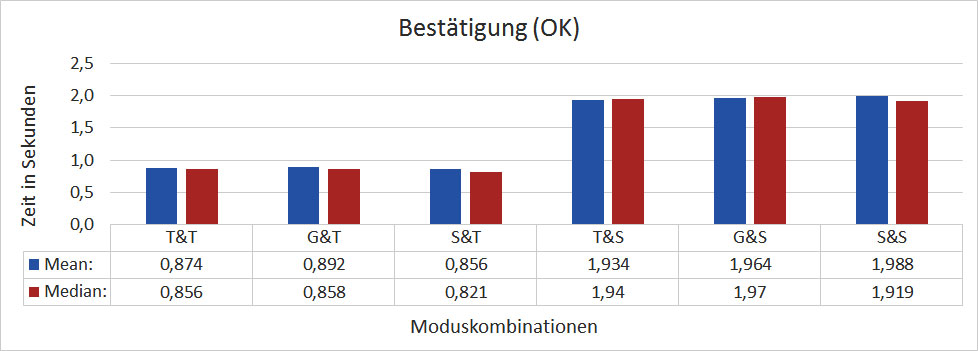
\includegraphics[width=1\textwidth]{img/B_OK.jpg}
  \caption{Durchschnittszeiten und Medianwerte in Sekunden für die Bestätigung der Texteingabe.}
  \label{fig:Bestaetigung_OK}
\end{figure} 

Im Anwendungsbeispiel Medien folgt im dritten Screen die Aktion direkte Inkrementation (Inkr. (d)) durch den Slider (siehe \fref{fig:Slider}) mit einem anschließendem Popup (siehe \fref{fig:Popup}). 
Auch hier ist das Laden der Szene der Startpunkt der Aktion. 
Sobald der Slider im gewünschten Bereich von 75-85\% losgelassen wird endet die Aktion und das Popup wird sichtbar. 
Das Ende der Aktion Inkr. (d) ist der Start der Bestätigungsaktion B. 
Diese endet mit der Selektion des Popups.
\begin{figure}[ht]
  \centering
  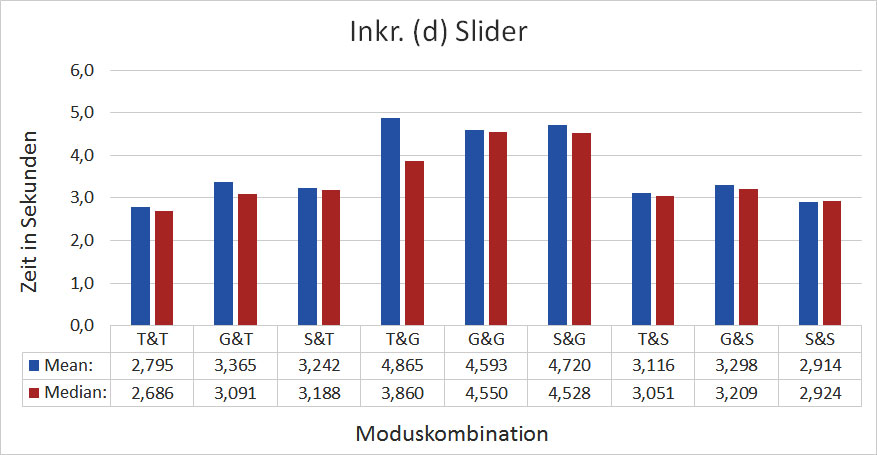
\includegraphics[width=1\textwidth]{img/Slider.JPG}
  \caption[Durchschnittszeiten für Inkr. (d)]{Durchschnittszeiten in Sekunden für die Aktion Slider von 50 auf 75 bis 85 Prozent für alle Moduskombinationen}
  \label{fig:Slider}
\end{figure} 
\begin{figure}[ht]
  \centering
  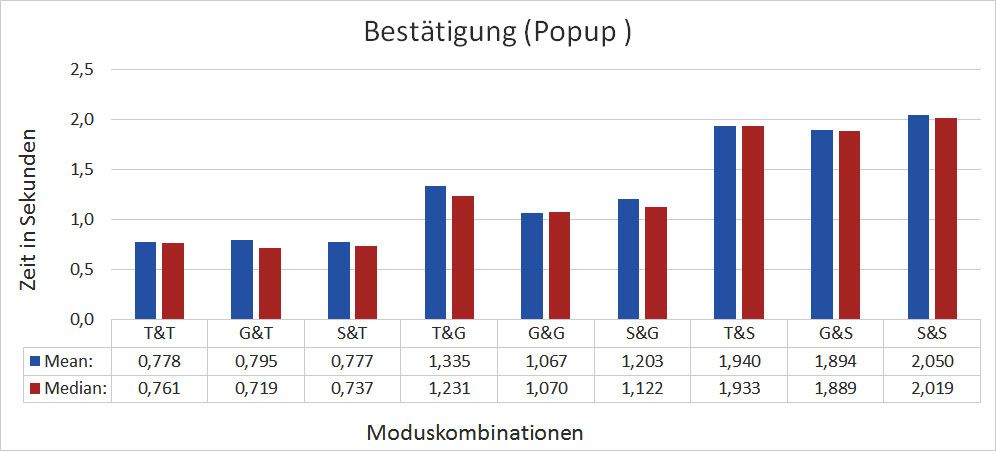
\includegraphics[width=1\textwidth]{img/PopupBestaetigung.JPG}
  \caption[Durchschnittszeiten für die Bestätigung des Popups]{Durchschnittszeiten in Sekunden für die Bestätigung des Popups für alle Moduskombinationen}
  \label{fig:Popup}
\end{figure} 
Auch bei den Zeiten für (Inkr. (d)) bestätigt sich erneut, dass die unimodalen Varianten schneller sind als die multimodalen Varianten. 
Bei dem anschließenden Popup hat der Moduswechsel bereits stattgefunden und es ist auch zu erkennen, dass sich die Zeiten hier zum vorherigen Modus nicht mehr so stark unterscheiden.

Als letzte Aktion bleibt noch die stufenweise Inkrementation Inkr. (s) im Anwendungsbeispiel Temperatur (siehe \fref{fig:SwipeKlima}). 
Der Startpunkt beginnt mit dem Laden der Szene für die Einstellung der Temperatur. 
Der erste Swipe endet genau wie bei der Listen-Navigation (L) mit dem Erreichen der nächsten Seite. 
Hier startet gleichzeitig der nächste Swipe, bis wir bei der gewünschten Seite mit dem dritten Swipe angekommen sind. 
Es folgt eine Verzögerung bis der Wert eingeloogt wird. 
Diese wird in die Gesamtzeit nicht miteinbezogen, da das Ziel bereits erreicht ist. 

Auch hier ist deutlich zu sehen, dass der erste Swipe am längsten dauert und Swipe 2 und 3 hingegen sehr ähnlich sind. 
Die unimodalen Varianten beim ersten Swipe sind ebenfalls schneller als bei den multimodalen Varianten.
\begin{figure}[ht]
  \centering
  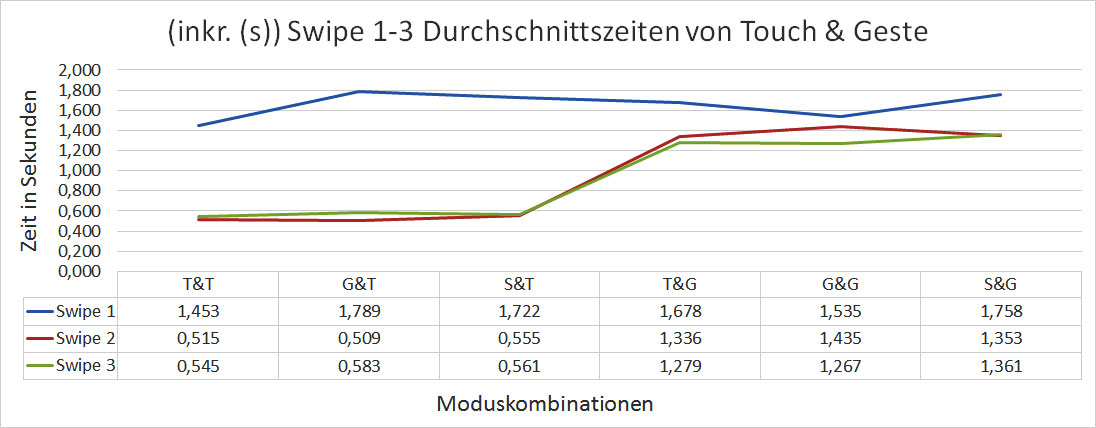
\includegraphics[width=1\textwidth]{img/Swipe1-3_Klima.JPG}
  \caption[Durchschnittszeiten für Inkr. (s)]{Durchschnittszeiten für Swipe 1, 2 und 3 in Sekunden der Wertinkrementation für die Moduskombinationen von Touch und Geste}
  \label{fig:SwipeKlima}
\end{figure} 

Wir haben jetzt unsere Aktionen ausgewertet und einen Blick auf die verschiedenen Zeiten geworfen, im folgenden werden die Zeiten auf  statistisch signifikante Unterschiede untersucht. 

\subsection[Statistische Tests]{Statistische Tests der Aktionszeiten}
Mit einer One-Way Repeated Measures ANOVA wurde mit Hilfe von SPSS für jede Aktion geprüft, ob der zweite Modus einen signifikanten Einfluss auf den ersten Modus hat und vor allem, ob der erste Modus einen signifikanten Einfluss auf den zweiten Modus hat. 
Die anhängige Variable war dabei der Modus (Touch, Geste und Sprache) und es wurden die wiederholten Messungen der Zeiten verglichen. 

Bei diesem Test muss beachtet werden, dass die Sphärizität nicht verletzt wird. 
\citet{field2002design} erklärt in seinem Buch "`How to Design and Report Experiments"' wie dies in SPSS berücksichtigt wird. 
Ist bei Mauchly's Test der Sphärizität das Ergebnis signifikant wird die Sphärizität verletzt und es muss eine Korrektur vorgenommen werden. 
Wir verwenden bei unseren Ergebnissen für eine Korrektur, die Greenhouse-Geisser Korrektur. 
Ist bei Mauchly's Test der Sphärizität das Ergbenis nicht signifikant, ist die Sphärizität auch nicht verletzt und es kann beim Test der Inner-Subjekt Effekten der Wert aus der Zeile entnommen werden, indem die Sphärizität angenommen wird \citep{field2002design}.

Diese Auswertung zur Überprüfung von signifikanten Unterschieden wurde für jede Aktion innerhalb ihrer Modalität überprüft. 
Die Ergebnisse werden im Abschnitt \ref{sec:Herleitung} präsentiert.
